\section{Markerless Recognition}

\subsection{Colour Search}
An application was designed, which would analyse the video feed from the Kinect. An initial, rudimentary, mechanism was used to highlight values in the output image on a binary basis: matches in white, the rest in black. A more efficient algorithm, if needed, would be put in place during any further development.\\
 
\begin{description}
\item[Capture] Frames captured from device
\item[Convert] Convert to HSL colour space, if required
\item[Search] Check very pixel value against target range
\item[Filter] Threshold data to remove noise, by keeping only pixels with a sufficient number of surrounding target pixels
\end{description} \\
 
Attaching a control to the original video feed allowed click-to-select and click-to-find functionality, which makes it significantly easier to obtain and then search for and refine the colour of an object.\\

\begin{description}
\item[Select] Click on video feed
\item[Search] Select search button
\item[Refine] Adjust colour components and variance
\end{description} \\

\begin{figure}
\begin{center}
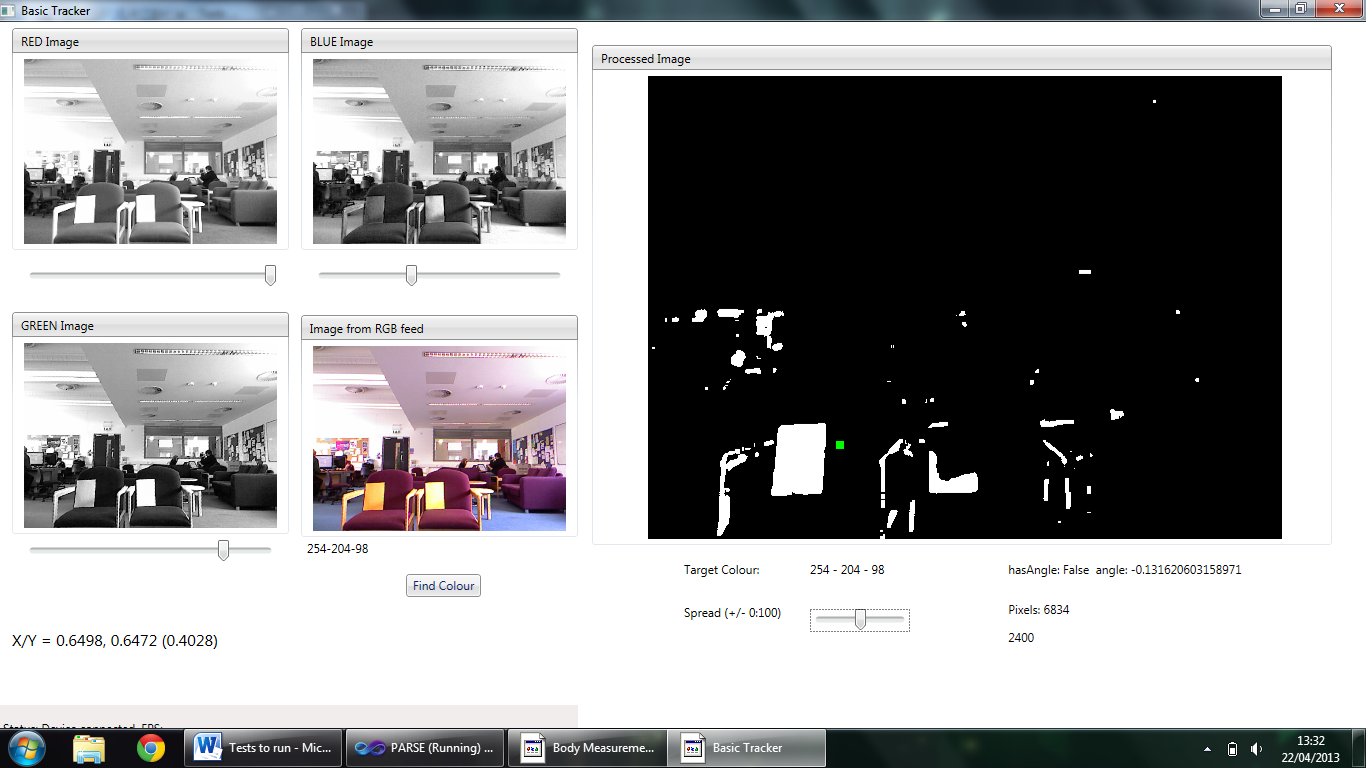
\includegraphics[scale=0.2]{zscreenshots/screenshot_testing_rgb_orange}
\caption{The RGB colour search test environment}
\end{center}
\end{figure} \\

\subsection{SURF}
The SURF implementation was incorporated as a visualisation method in the main application, which allowed simple access to the Kinect and the possibility for further development later. Due to the computational complexity, it was not possible to run SURF in real time on the hardware available. Each SURF run takes a few seconds, which makes video or real-time testing non-viable. The SURF classifier was therefore tested only on static images, by creating a mechanism by which two frames were captured in a clear, guided process on-screen.\\

The default parameters were investigated, and the setup was deemed sufficient for the tests. Minor alterations were tested off-record, with little to report. \\

The program was configured to output a single image containing, on the right side, the target image with its features highlighted, and on the left side the input image with its features highlighted. Any correspondences between the two images' features are indicated with lines, and any target identified is indicated by a rectangle.\\

\begin{figure}
\begin{center}
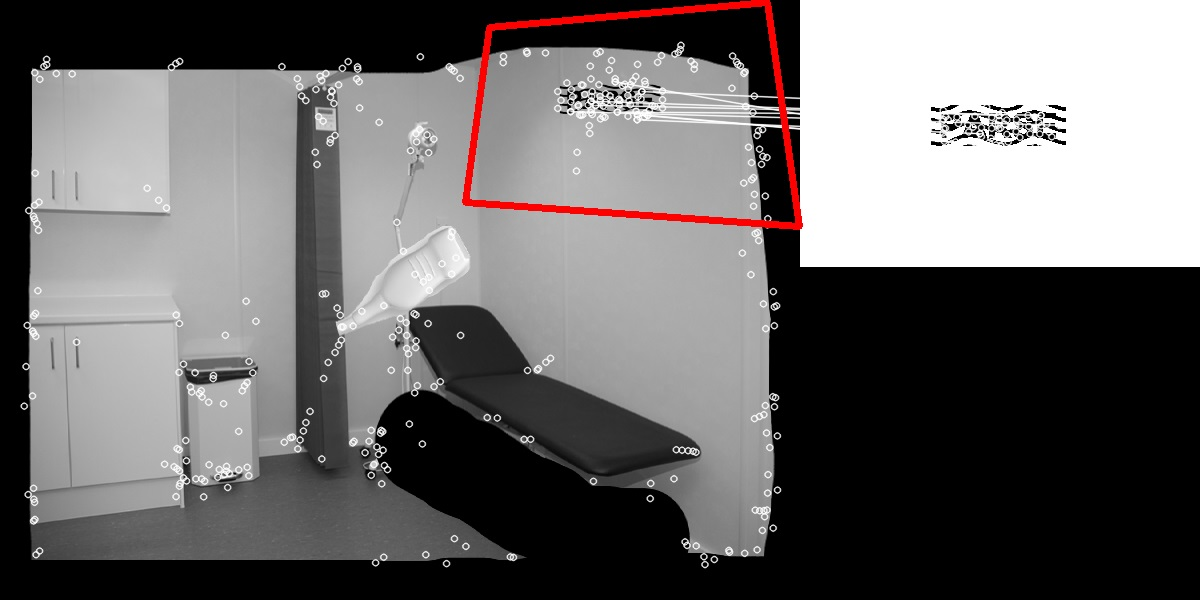
\includegraphics[scale=0.25]{zscreenshots/SURF-Example.jpg}
\caption{An output image, with the found target indicated}
\end{center}
\end{figure}

\subsection{Haar}
The generation of the Haar classifier was to be fraught with complex procedures and intricate setup details. It took several weeks’ research and development to train a classifier at all, before testing could begin.\\

Limitations to this progress were numerous. For classifier use, the PCL library imports a classifier from a file, which is generated externally. To train the classifier, a precise setup must be created and then generated through use of an executable via an obscure command line process. Further, the training process requires large numbers of training images. The documentation suggested minimal numbers in the order of thousands; a quantity which would take quite some time to collect.\\

The first experiment was, therefore, to find the minimum number of samples required to find a simple object. An application was created to allow the import, classification, and export of images into the correct formats and directory structures required for the training process. A sample of fifty positive, classified images and fifty negative images was found to be sufficient to generate a classifier.\\

\subsection{Final Scan Process}
The final implementation, achieved after testing the tracking methodologies, used the colour space search in RGB format. We combined the RGB tracking with positioning components and a carefully designed workflow to create the final process. \\

\begin{itemize}
\item First, the operator and patient enter the field of view. Once the Kinect detects two skeletons, we search for the scanner using the RGB tracking mechanism.
\item Utilising the Kinect's skeletal data, the program searches for hands within a threshold distance of the scanner. Once one is found, that identifies that skeleton as the operator; and thus the other as the patient.
\item To capture the scan location, the operator need only hold the scanner still for a few seconds in order to trigger the capture routine. 
\end{itemize} \\

Looking ahead, the capture routine was engineered to fire an event within the C# runtime, which allows entities outside of the tracking class to be notified of the capture signal. This event could therefore be captured by some process intended to action data capture from a real sensing device. \\

\subsection{Coordinate Systems}
A key problem which was to be solved was the translation of the image-relative position of the sensor (in image coordinates) into real-world / skeletal coordinates. The coordinate systems do not align easily, nor exactly due to the physical offset in position between the depth and optical cameras. The Kinect API provides a set of coordinate space translations, but only into the RGB space, rather than from it. \\

To obfuscate matters further, the skeletal (real-world) coordinate system used by the Kinect uses ranges of -2.2 to +2.2 in the x axis, and -1.6 to 1.6 in the y axis.\\

The final solution used a basic trigonometric model, at fixed depth, because it was not possible to find the correlating depth value for a given RGB image pixel: \\

\begin{equation}
Real X = (((depth * 2 * tan(57) * X) / 640) - 2.2) * 1000
\label{Conversion of x coordinates from image into real space}
\end{equation} \\

\begin{equation}
Real Y = (((depth * 2 * tan(21.5) * (Y - 240)) / 480) + 1.05 ) * 1000
\label{Conversion of y coordinates from image into real space}
\end{equation} \\

\subsection{Skeleton-relative Positioning}
Following finding the location of the scanner in image coordinates, the location needs to be captured as a skeleton point relative to skeleton key points. For this purpose, the aim is to find the scanner location relative to the skeleton joints nearest to it.\\

The initial method for achieving this was implemented by using Pythagoras Theorem to calculate the distance of the scanner position relative to all joints. The joint that appeared to be the closest to the position was chosen and the scanner position was stored by using the difference between its coordinates and the coordinates of the closest joint. Even though this method appeared to be mostly adequate in our experiments, it was decided to implement some additional filtering of the joints before selecting the nearest one, in order to avoid errors that could potentially arise in situations where the body-type of the patient is very different to the ones that this method was being tested with.\\

The additions to the original method include finding the area around which the scan was made, from one of three main areas: legs, arms and chest. The division of the body into these areas is performed based on the 3 hip joints and the shoulders. Anything under the hip joints is classified as part of the legs and anything on the left and right of each of the left and right hips respectively is classified as arms. To confirm the arms, the shoulders are used as well. Following this division, if the scanner's location is on the chest area, the original method using Pythagoras Theorem will be applied, excluding all joints on the arms and legs, but finding the distance of the location from 3 joints instead of one, to improve accuracy of repositioning. If the scanner is on the legs or arms, the specific bone it is on will be found first, by comparing the position with the y of the joints of the legs or the x of the joints of the arms. Once that is determined and we have the 2 joints that make up the bone found, the distance of the scanner's coordinates from the coordinates of those joints is stored.\\

\subsection{Skeleton Identification}
Originally, it was intended that the Kinect skeletons of the operator and patient be intuitively identified by some measure independent the scan process, i.e. they should not have to do anything to identify themselves. This process was to be enabled by utilising the known locations of the scanner and the skeletons: the hand closest to the scanner (and within some threshold) must be that of the operator.\\

This mechanism proved to be problematic, however. The relatively poor reliability of the scanner tracking and of the hand tracking (from the Kinect API) meant that the process often took several seconds before the coordinates aligned sufficiently. A confirmation dialog was introduced during development, but the use of this caused yet more problems, as upon the operator's return to the frame they were allocated a new trackingID.\\

The final solution, although not ideal, was to have the operator stand to the left of the patient at the beginning of the scan process. This allowed for near-instant identification, saving up to thirty seconds against the previous method.\\
